\documentclass{article}
\usepackage[margin=2.5cm]{geometry} % Set margins
\usepackage{graphicx}
\usepackage[absolute]{textpos} % Enable absolute positioning
\usepackage{titlesec} % Package for controlling section title appearance
\usepackage[scaled]{helvet}
\usepackage[T1]{fontenc}
\usepackage{fancyhdr}

\usepackage{url} % Load the url package

% Set up hyperref
\usepackage{hyperref}
\hypersetup{
    colorlinks=true,
    linkcolor=blue,
    urlcolor=blue,
    linkbordercolor={0 0 1}
}

% Set up references
\usepackage[
    backend=biber,             % Use biber backend (an external tool)
    sorting=none,              % Enumerates the reference in order of their appearance
    style=authoryear           % Choose here your preferred citation style
]{biblatex}
\addbibresource{bibliography.bib} % The filename of the bibliography
\usepackage[autostyle=true]{csquotes} 
                               % Required to generate language-dependent quotes 
                               % in the bibliography

\setlength{\TPHorizModule}{1cm} % Set horizontal unit of measure
\setlength{\TPVertModule}{1cm} % Set vertical unit of measure
\setlength{\parindent}{0pt}

\renewcommand{\familydefault}{\sfdefault}

\makeatletter
\renewcommand{\maketitle}{
  \begin{flushleft} 
    \Large\textmd{\@title} 
    \par
  \end{flushleft}
}
\makeatother

% Define style of sectiontitles
\titleformat{\section}
  {\normalfont\large\mdseries}{\thesection}{1em}{}

% Set up fancyhdr
\fancyhf{} % Clear all headers and footers
\renewcommand{\headrulewidth}{0pt} % Remove the header rule
\rfoot{\thepage} % Place the page number in the right footer
\pagestyle{fancy}


%%%%% Title %%%%%
\title{NDVI calculation using Sentinel-2 data and Python}

\begin{document}

%%%%% Header %%%%%
\begin{textblock}{1}(2.5,1) % Position 1cm from left and 1cm from top
        \includegraphics[width=6cm]{logo.jpg} % Add logo
\end{textblock}

\begin{textblock}{6}(13,1) % Position 14cm from left and 1cm from top
        \raggedleft
        Julian Kraft UI22\\
        Remote Sensing\\
        \today
\end{textblock}

\vspace*{1.5cm}

%%%%% Document %%%%%

\maketitle

\section*{Introduction}

The Normalized Difference Vegetation Index (NDVI) is a widely used index to monitor vegetation health and growth. 
It is calculated from the red and near-infrared bands of satellite imagery. The NDVI values range from -1 to 1, 
where values close to 1 indicate healthy vegetation and values close to -1 indicate no vegetation. In this report, 
the calculation using Sentinel-2 satellite data and Python is described. 
The data processing was done for the area of the Kanton of Schaffhausen in Switzerland. The area is defined by the bounding box
(West: 8.3, South: 47.53, East: 8.9, North: 47.84, ESPG:4326). 
The temporal extent covers the summer months (June, July, August) of the years 2017 to 2023.
To solve this task,
three different Remote Sensing products are used: Sentinel-2 Level-2A data bands B04 (Red) and B08 (NIR) and the
preprocessed Scene Classification Layer (SCL). In this report the focus is on how the data was obtained and processed
and how the created NDVI product looks like for a single time frame.\\

For the next step, namely task 2, the idea is to analyze the data over time. The NDVI for itself provides limited information
about the actual vegetation health and growth, since the values are relative. Therefore, the plan is to calculate the 
deviation from the mean NDVI over the whole time analyzed for each pixel on every time frame. This needs to be further
elaborated and tested.\\

\section*{Methods}

To process and download the data, the \href{https://openeo.dataspace.copernicus.eu/}{OpenEO} platform was used. 
There is a great advantage in using platforms like this, since they provide a lot of functionalities to process date in the cloud
before downloading only the needed result. The platform provides a Python API, which was used to access the data and process it.
It is important to split the processing into smaller steps, since the data is too large to be processed at once.
In this case it was done month by month.
The code is available on \href{https://github.com/juliankraft/RemoteSensing_Task01}{GitHub}. 
Only frames with less than 85\% cloud cover were used.\\

The NDVI was calculated using the following formula \autocite{ndvi_sentinelhub}:\\

\begin{equation}
    NDVI = \frac{NIR - RED}{NIR + RED}
\end{equation}\\

After calculating the NDVI, the values were masked using the SCL layer. All pixels not classified as vegetation were set to not 
available (nan) in order for them not to be considered in the analysis. This solves the problem of having NDVI values for clouds as well
as NDVI values for water bodies, urban areas, etc. The final NDVI product was then downloaded as Data Cube with the dimensions
time, x, y and the coordinate system ESPG:32632. The data cube was saved as a NetCDF file.\\

\section*{Results}

In Figure \ref{fig:ndvi_plot} the NDVI for the Kanton of Schaffhausen for a single time frame is shown.
There are some plain white areas where no values are available. The values for the NDVI range from 0.2 to 0.9.
This represents only a sample of the generated data. For every Image of Sentinel-2 with a cloud coverage of less than 85\%
during the defined spatial and temporal extent - data is available and ready for further analysis.

\begin{figure}[h]
  \centering
  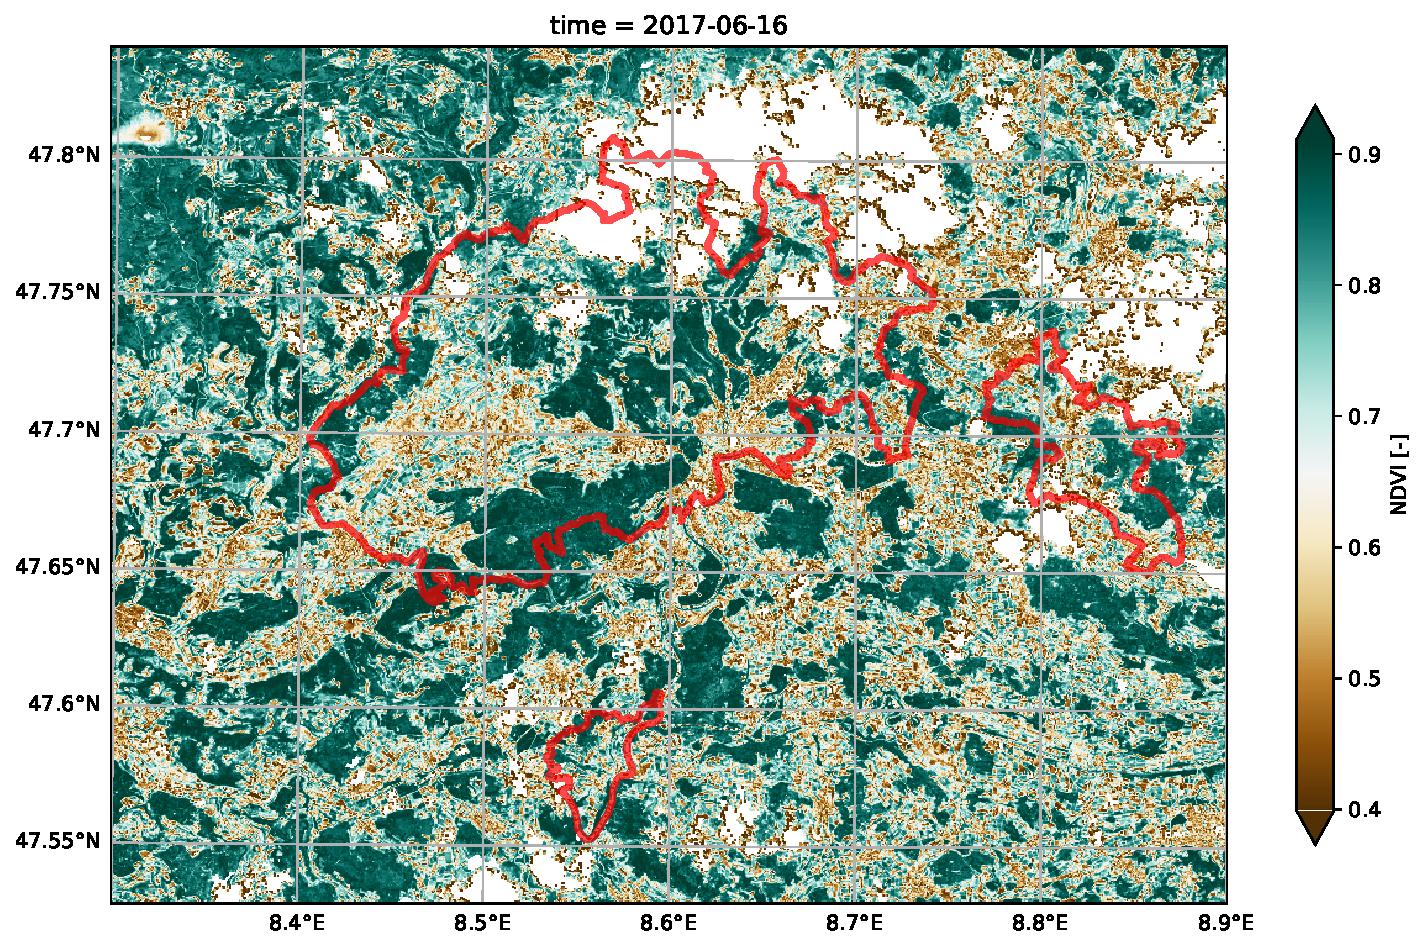
\includegraphics[width=0.8\textwidth]{ndvi_plot.pdf}
  \caption{Plot of the NDVI for the Kanton of Schaffhausen for a single time frame. The red line represents the boarder of the Kanton.}
  \label{fig:ndvi_plot}
\end{figure}


\section*{Discussion}

The dark green areas in Figure \ref{fig:ndvi_plot} represent especially dense and healthy vegetation. The area more or less corresponds to the forested area.
The values range only from 0.2 to 0.9, wich is most likely due to the fact that only vegetation pixels are considered
and the conditions for plant growth must have been good. Anyhow it is difficult to explain with no further investigation.
This is something that will be analyzed in more detail before taking the task further.

 

\vfill

\printbibliography

% declare AI assistance
\section*{Declaration of AI Assistance}
ChatGPT was used to answer a broad variety of questions concerning Python and LaTeX code\\
GitHub copilot was used to assist while writing the report and coding

\section*{Code}
All code is available on \url{https://github.com/juliankraft/RemoteSensing_Task01}

\end{document}